%%%%%%%%%%%%%%%%%%%%%%%%%%%%%%%%%%%%%%%%%%%%%%%%%%%%%%%%%
%%             东南大学数电实验报告 LaTeX 模板
%%                SEU-Circuit-Report.cls
%% https://github.com/Teddy-van-Jerry/SEU_Digital_Report
%% ======================================================
%% 版本信息:
%% v1.0 (Nov. 07, 2021)
%% ------------------------------------------------------
%% 模板制作:
%% Teddy van Jerry, (me@teddy-van-jerry.org)
%% * GitHub: https://github.com/Teddy-van-Jerry
%% * Website: https://teddy-van-jerry.org
%% * Blog: https://blog.teddy-van-jerry.org
%% ------------------------------------------------------
%% 使用说明:
%% 1. 编译使用 XeLaTeX 和 Biber
%% 2. 报告基本信息通过修改导言区以 exp 开头的命令
%% 3. 参考文献位于 ref/ref.bib
%% 4. 报告模板依据 MIT License 开源共享
%% ------------------------------------------------------
%% Copyright 2021 (c) Teddy van Jerry
%%
%% Permission is hereby granted, free of charge, to any
%% person obtaining a copy of this software and
%% associated documentation files (the "Software"), to
%% deal in the Software without restriction, including
%% without limitation the rights to use, copy, modify,
%% merge, publish, distribute, sublicense, and/or sell
%% copies of the Software, and to permit persons to whom
%% the Software is furnished to do so, subject to the
%% following conditions:
%%
%% The above copyright notice and this permission notice
%% shall be included in all copies or substantial
%% portions of the Software.
%% 
%% THE SOFTWARE IS PROVIDED "AS IS", WITHOUT WARRANTY OF
%% ANY KIND, EXPRESS OR IMPLIED, INCLUDING BUT NOT
%% LIMITED TO THE WARRANTIES OF MERCHANTABILITY, FITNESS
%% FOR A PARTICULAR PURPOSE AND NONINFRINGEMENT. IN NO
%% EVENT SHALL THE AUTHORS OR COPYRIGHT HOLDERS BE LIABLE
%% FOR ANY CLAIM, DAMAGES OR OTHER LIABILITY, WHETHER IN
%% AN ACTION OF CONTRACT, TORT OR OTHERWISE, ARISING
%% FROM, OUT OF OR IN CONNECTION WITH THE SOFTWARE OR THE
%% USE OR OTHER DEALINGS IN THE SOFTWARE.
%%%%%%%%%%%%%%%%%%%%%%%%%%%%%%%%%%%%%%%%%%%%%%%%%%%%%%%%%%

%% 使用实验报告模板类(字体大小 11pt 约为五号字)
\documentclass[11pt]{SEU-Digital-Report}

%%%%%%%%%%%%%%%%%%%% 报告基本信息 %%%%%%%%%%%%%%%%%%%%
\expno{九} % 实验序号
\expname{时钟实验} % 实验名称
\expauthor{薛宇飞} % 姓名
\expID{04020235} % 学号
\expmates{} % 同组
\expmatesID{} % 学号(同组)
\expmajor{信息工程} % 专业
\explab{金智楼硬件实验室} % 实验室
\expdate{\today} % 实验日期
\expreportdate{\today} % 实验日期
\expgrade{} % 成绩评定
\exptutor{裴文江} % 评阅教师
%%%%%%%%%%%%%%%%%%%%%%%%%%%%%%%%%%%%%%%%%%%%%%%%%%%%
% \usepackage{xeCJK}
\usepackage{threeparttable} %table添加注释
\usepackage{colortbl}
\newcommand{\grayrow}{\rowcolor[rgb]{ .906, .902, .902}}
\usepackage{xcolor}  % tikz画图
\usepackage{tikz}  
\usetikzlibrary{arrows,shapes,chains} 
\usepackage{pgfplots}
\pgfplotsset{compat=1.11}

%% 报告正文
\begin{document}

% 打印封面页
\exptitlepage

\tableofcontents
\newpage

\section{实验目的与内容}       
\begin{enumerate}
    \item 结合实验教材\cite{book,guide},熟悉系统功能调用\texttt{INT 21H}的有关功能。
    \item 编写时钟程序。
\end{enumerate}

\section{\textcolor{red}{预习报告}}
\subsection{实验任务}       
\begin{enumerate}
    \item 执行时钟程序时,屏幕上显示提示符“:” ,由键盘输入当前时、分和秒值,即\texttt{XX:XX:XX√},随即显示时间并不停地计时。
    \item 当有键按下时,立即停止计时,返回\texttt{DOS}。
\end{enumerate}

\subsection{实验原理}
首先利用系统调用\texttt{INT 21H}中\texttt{02H}功能,在\texttt{CRT}上显示一个提示符“:”,要求用户从键盘输入时钟初值(即当前时间),其输入格式为\texttt{XX}(时):\texttt{XX}(分):\texttt{XX}(秒)\texttt{√}。然后利用\texttt{0AH}功能调用接收从键盘输入的字符串,并将接收的字符串存入到缓冲区。

在利用\texttt{0AH}功能调用前要设置一个缓冲区,在调用时,用\texttt{DX}作为输入缓冲区的指针,由键盘输入的字符存入该缓冲区,直至遇到回车键为止。
程序中把输入的‘时’、‘分’、‘秒’初值分别从输入缓冲区中取出,各自放在一个寄存器中,然后调用一个延时1秒钟的子程序,每过1秒使秒值增1,然后检查是否已为60秒,若不是则转显示;若是,则使秒值为0,分值增l,检查是否已为60分,若不是则转显示,若是,则使分值为0,时值增1,接着检查时值是否为24小时,若不是则转显示,若是,则使时值为0,接着也是转显示。
若使程序运行停止,只要有键按下,即可返回\texttt{DOS}。下面列出两种判别是否有键按下的方法:
\begin{enumerate}
    \item 读键扫描码:\\
\begin{lstlisting}[language={[x86masm]Assembler},title=code]
        IN    AL,60H     ;读键扫描码
        TEST  AL, 80H  
        JZ    AAA        ;有键按下,就转AAA
            :
            :
    AAA:MOV AH,4CH
        INT   21H  
\end{lstlisting}
    \item 调用\texttt{INT 21H}中\texttt{06}功能:\\
\begin{lstlisting}[language={[x86masm]Assembler},title=code]
        MOV   AH,06
        MOV   DL,0FFH        ;判断是否有键按下,有键按下则转AAA
        INT   21H   
        JNZ   AAA
            :
            :
    AAA:MOV AH,4CH
        INT   21H
\end{lstlisting}
\end{enumerate}

\subsection{流程框图}
实验流程图如图 \ref{fig:process}所示。
\begin{figure}[htbp]
    \centering
    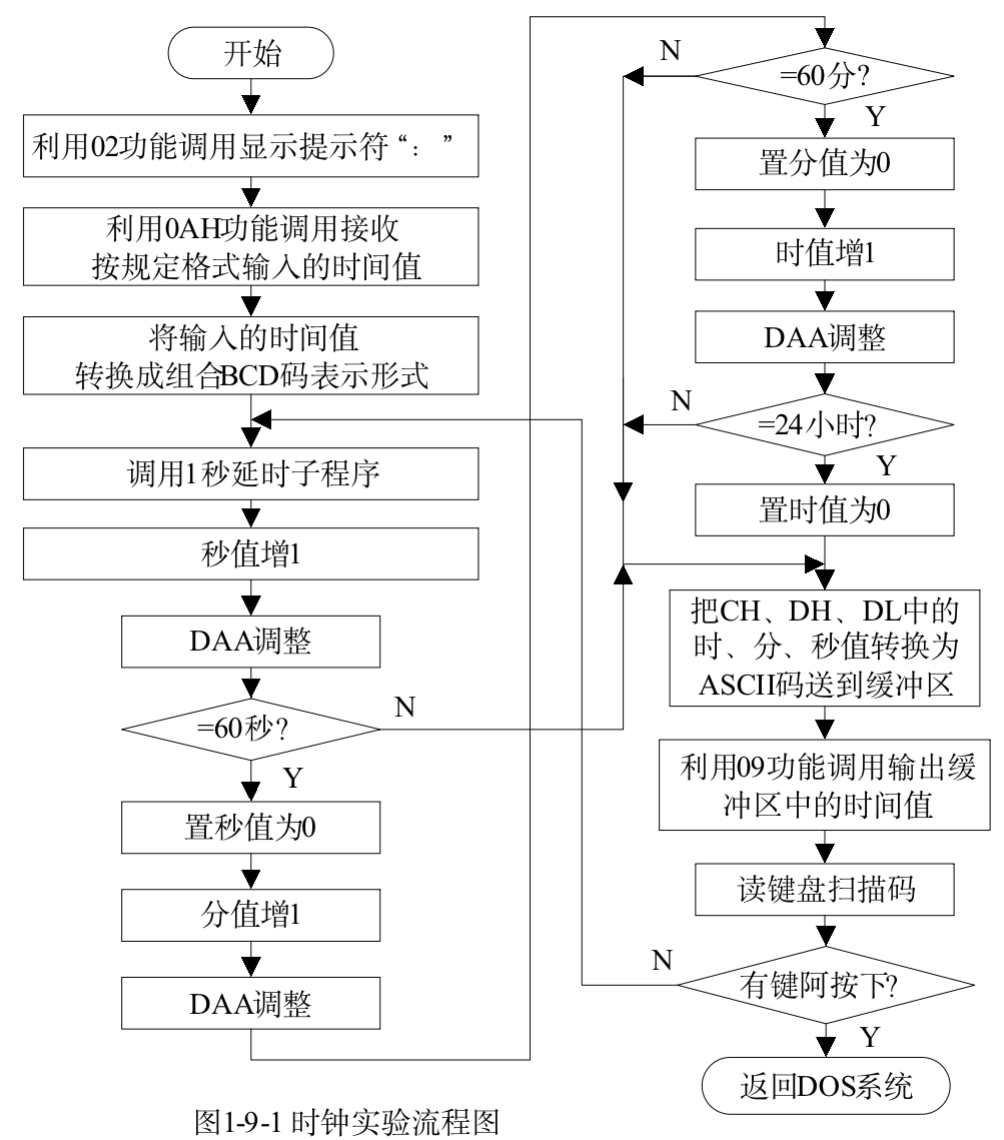
\includegraphics[width=0.7\textwidth]{fig/process.png}
    \caption{}
    \label{fig:process}
\end{figure}

\subsection{实验可能用到的代码}
延时1秒子程序\texttt{DELAY}:
\begin{lstlisting}[language={[x86masm]Assembler},title=delay]
    DELAY PROC
          PUSH   CX
          PUSH   AX
          MOV    CX,0FFFFH
    GOON: DEC    CX
          JNE    GOON
          POP    AX
          POP    CX
          RET
    DELAY ENDP
\end{lstlisting}

\subsection{实验代码}
时钟实验代码如下(包括三个附加程序):
\begin{lstlisting}[language={[x86masm]Assembler},title=CLK]
    DATA SEGMENT
    TIME_IN       DB 9,?,9 DUP(?),'$'   ;缓冲区格式要求:
                                        ;允许最大字符数(带回车)、
                                        ;实际字符数(系统自动写入回车)、
                                        ;缓冲区、0DH
    PRINT_ETR     DB 0DH,0AH,'$'        ;设置一回车输出串,
                                        ;在“:”显示后输出,换行缩进
                                        ;汇编里回车是回到本行首位,
                                        ;换行是到下一行同样位置
    TIME_CHG      DB ?,?,?              ;设置一时间存储空间,
                                        ;便于在执行时间的ASCII码与压缩BCD码
    WRONG_VALUE   DB 'Wrong value! Try again','$'                           ;错误类型1
    WRONG_NUMBER  DB 'The input must be colons or number! Try again','$'                           ;错误类型2
    DATA ENDS

    STACK SEGMENT
    STACK_SPACE   DB 8 DUP(?)           ;开辟栈段,
                                        ;dos调用delay以及‘分’、‘秒’
                                        ;保护会用到栈段
    STACK ENDS

    CODE SEGMENT
    ASSUME CS:CODE,DS:DATA,ES:DATA
    START: 
        MOV AX,DATA
        MOV DS,AX
        MOV ES,AX                   ;设置DS段和ES段的段地址
    INPUT: 
        MOV DL,':'                  ;显示时间输入提示符号“:”
        MOV AH,02H
        INT 21H
        LEA DX,PRINT_ETR            ;附加任务1:
                                    ;显示“:”后输出一个回车,
                                    ;便于时间的正确输出
        MOV AH,09H
        INT 21H
        LEA DX,TIME_IN              ;接收输入的时间
        MOV AH,0AH
        INT 21H
    LENTH_TEST:                     ;长度测试
        MOV AL,TIME_IN+1            ;实际键入字数 
        CMP AL,08H                  ;和8比较,不相等跳转到 WRONG_INPUT
        JNE WRONG_INPUT_2
    FORMAT_TEST:                    ;格式测试
        MOV AL,TIME_IN+4            ;格式:XX:XX:XX
        CMP AL,':'
        JNE WRONG_INPUT_2
        MOV AL,TIME_IN+7
        CMP AL,':'
        JNE WRONG_INPUT_2
    INIT_LOW_LIMIT_TEST:
        LEA SI,TIME_IN+2
        MOV CL,03H                  ;循环3次
    LOW_LIMIT_TEST:
        MOV AL,[SI]		
        MOV AH,[SI+1]
        CMP AL,30H                  ;字符‘0’的ASCII码是30,不能小于0
        JB WRONG_INPUT_2            ;无符号小于则跳转
        CMP AH,30H                  ;字符‘0’的ASCII码是30,不能小于0
        JB WRONG_INPUT_2            ;无符号小于则跳转
        ADD SI,0003H
        LOOP LOW_LIMIT_TEST
    INIT_HIGH_LIMIT_TEST:
        LEA SI,TIME_IN+2
        MOV CL,03H
    HIGH_LIMIT_TEST:
        MOV AL,[SI]		
        MOV AH,[SI+1]
        CMP AL,39H                  ;字符‘9’的ASCII码是39,
                                    ;不能超过9,先得是个数字
        JA WRONG_INPUT_2            ;无符号大于则跳转
        CMP AH,39H                  
        JA WRONG_INPUT_2
        ADD SI,0003H
        LOOP HIGH_LIMIT_TEST
    HOUR_HIGH_TEST:
        MOV AL,TIME_IN+2
        CMP AL,32H                  ;字符‘2’的ASCII码是32,
                                    ;‘时’第一位不能超过2,
                                    ;‘分’和‘秒’同理
        JA WRONG_INPUT_1
    HOUR_FULL_HIGH_TEST:
        MOV AL,TIME_IN+3
        MOV AH,TIME_IN+2
        CMP AX,3233H                ;字符‘0203’的ASCII码是3233
        JA WRONG_INPUT_1
    MINUTE_TEST:
        MOV AL,TIME_IN+5
        CMP AL,35H
        JA WRONG_INPUT_1
    SECOND_TEST:
        MOV AL,TIME_IN+8
        CMP AL,35H
        JA WRONG_INPUT_1
        JMP INIT_IN                 ;检查完进行一个时间数值的调整
    WRONG_INPUT_1:
        LEA DX,WRONG_VALUE
        MOV AH,09H
        INT 21H
        JMP INPUT                   ;有错误需要重新输入
    WRONG_INPUT_2:
        LEA DX,WRONG_NUMBER
        MOV AH,09H
        INT 21H
        JMP INPUT                   ;有错误需要重新输入
    INIT_IN:
        LEA SI,TIME_IN+2            ;时间ASCII码转化为压缩BCD码的初始化
        LEA DI,TIME_CHG
        MOV BL,03H                  ;时、分、秒各一次
        MOV CL,04H
    TRANS_IN:                       ;结果是TIME_CHG中分别放着
                                    ;时、分、秒的BCD码
        MOV AL,[SI]		            ;移入相应时间量度的数值
        MOV AH,[SI+1]
        SHL AH,CL                   ;左移4位,把ASCII的30挪掉
                                    ;让时间的两位挨在一起
        ROL AX,CL                   ;右移4位,把挨在一起的高低位挪进AL
        MOV [DI],AL
        DEC BL                      ;计算换算次数,判断是否换算完毕
        CMP BL,00
        JE GETTIME                  ;若换算完毕,进入下一部分操作
        ADD SI,0003H                ;指向下一时间单位的缓冲区存储空间
        INC DI                      ;时间储存区加1
        JMP TRANS_IN                ;循环进行换算操作
    GETTIME:
        LEA DI,TIME_CHG             ;将时间的压缩BCD码赋给相应的寄存器
        MOV CH,[DI]
        MOV DH,[DI+1]
        MOV DL,[DI+2]
        JMP PRINT
    SECPLUS:
        CALL DELAY                  ;执行延时1秒子程序
        MOV AL,DL                   ;秒+1,并进行压缩BCD码加法调整,
                                    ;计算完毕放回相应寄存器
        ADD AL,01
        DAA
        MOV DL,AL
    SECOND:
        CMP DL,60H                  ;判断秒值与60的大小关系,
                                    ;小于则跳转执行输出初始化
        JB INIT_OUT                 ;进行秒的进制调整,无符号小于则跳转
        MOV DL,00                   ;秒值置0
        MOV AL,DH                   ;分+1,并进行压缩BCD码加法调整,
                                    ;计算完毕放回相应寄存器
        ADD AL,01
        DAA
        MOV DH,AL
    MINUTE:
        CMP DH,60H                  ;判断分值与60的大小关系,
                                    ;小于则跳转执行输出初始化
        JB INIT_OUT                 ;进行分的进制调整
        MOV DH,00                   ;分值置0
        MOV AL,CH                   ;时+1,并进行压缩BCD码加法调整,
                                    ;计算完毕放回相应寄存器
        ADD AL,01
        DAA
        MOV CH,AL
    HOUR:
        CMP CH,24H                  ;判断时值与24的大小关系,
                                    ;小于则跳转执行输出初始化
        JB INIT_OUT                 ;进行时的进制调整
        MOV CH,00                   ;时值置0
    INIT_OUT:
        LEA DI,TIME_CHG             ;时间输出的初始化
        LEA SI,TIME_IN+2
        MOV [DI],CH                 ;将各时间单位数值对应存放进
                                    ;TIME_CHG中,以备码制转换
        MOV [DI+1],DH
        MOV [DI+2],DL
        MOV BL,03H
        MOV CL,04H
    TRANS_OUT:
        MOV AL,[DI]                 ;移入相应时间量度的压缩BCD码
        MOV AH,33H                  ;通过移位操作,可以得到对应的ASCII码
        ROR AX,CL
        ROR AH,CL
        MOV [SI],AL                 ;将转换的ASCII码存入缓冲区
        MOV [SI+1],AH
        DEC BL                      ;计算换算次数,判断是否换算完毕
        CMP BL,00
        JE PRINT                    ;若换算完毕,进入下一部分操作
        ADD SI,0003H                ;指向下一时间单位的缓冲区存储空间
        INC DI
        JMP TRANS_OUT               ;循环进行换算操作
    PRINT: 
        MOV BX,DX                   ;保护计算得到的分、秒信息
        LEA DX,TIME_IN+2            ;输出时间
        MOV AH,09H
        INT 21H
    IS_PUSH: 
        MOV AH,06                   ;判断是否有按键按下
        MOV DL,0FFH       
        INT 21H
        JNZ LAST                    ;若有按键按下,执行LAST
        MOV DX,BX                   ;若没有按键按下,则恢复分、秒信息,
                                    ;继续进行计时
        JMP SECPLUS           
    LAST:
        MOV AH,4CH                  ;返回dos,结束程序
        INT 21H
        HLT                         ;处理器进入暂停状态
    DELAY PROC NEAR                 ;延时1秒子程序     
        PUSH CX
        PUSH AX
        PUSH DX
        PUSH BX
        MOV AH,2CH                  ;读取当前时间,
                                    ;CH:小时;CL:分;DH:秒;
                                    ;DL:百分之一秒
        INT 21H
        MOV BH,DH                   ;将当前秒数存在BH中
        MOV AH,2DH                  ;设置时间
        INT 21H
    READ:
        MOV AH,2CH
        INT 21H
        CMP DH,BH                   ;比较两个时间的秒数,若相等则继续循环
        JE READ                     ;否则则经过了一秒
        POP BX
        POP DX
        POP AX
        POP CX
        RET
    DELAY ENDP
    CODE ENDS
    END START
\end{lstlisting}

\section{实验效果图}
实验中错误提示如图 \ref{fig:wrong},正确显示结果如图 \ref{fig:right}。
\begin{figure}[htbp]
    \centering
    \subfloat[错误提示1]{
        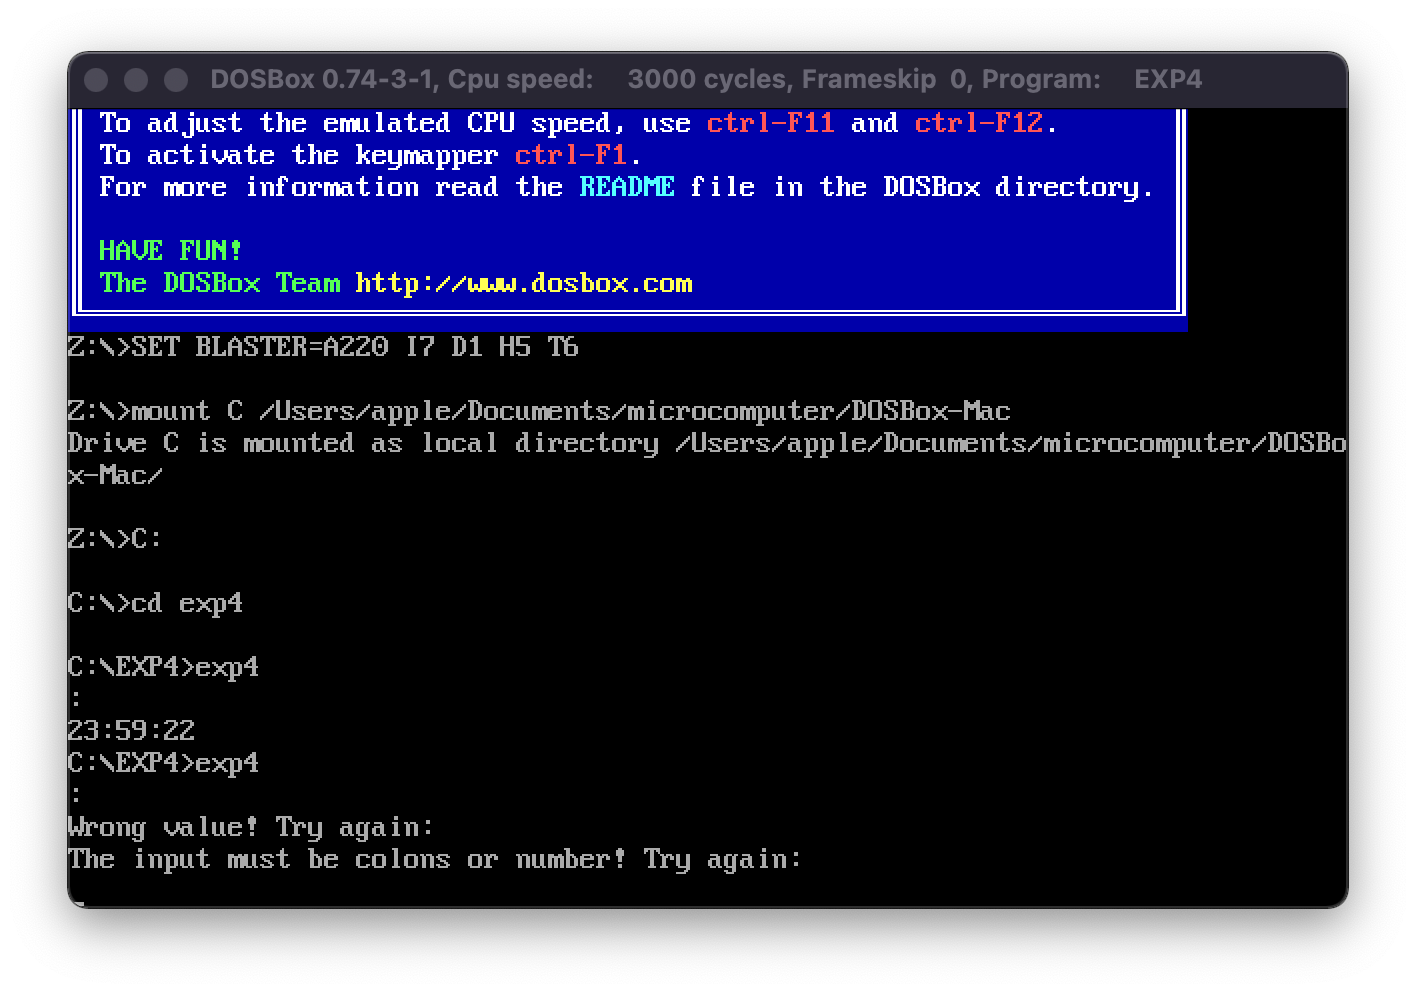
\includegraphics[width=0.4\textwidth]{fig/rlt00003.png}
        \label{subfig:wrong1}
    }
    \subfloat[错误提示2]{
        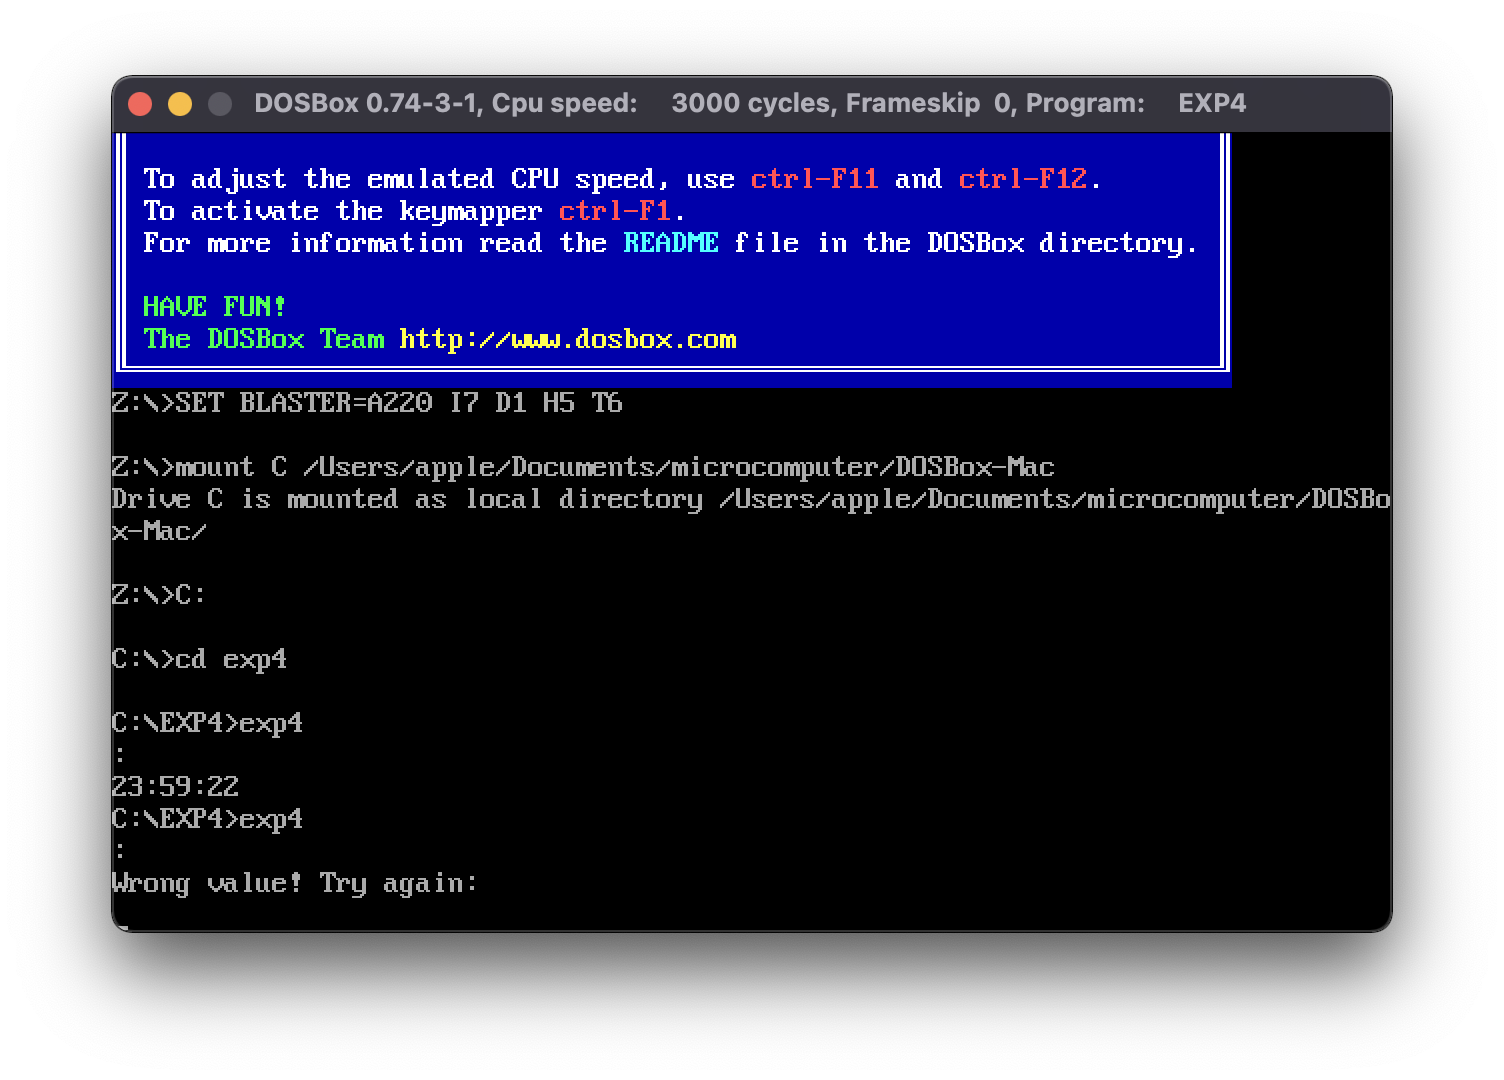
\includegraphics[width=0.4\textwidth]{fig/rlt00001.png}
        \label{subfig:wrong2}
    }
    \caption{}
    \label{fig:wrong}
\end{figure}

\begin{figure}[htbp]
    \centering
    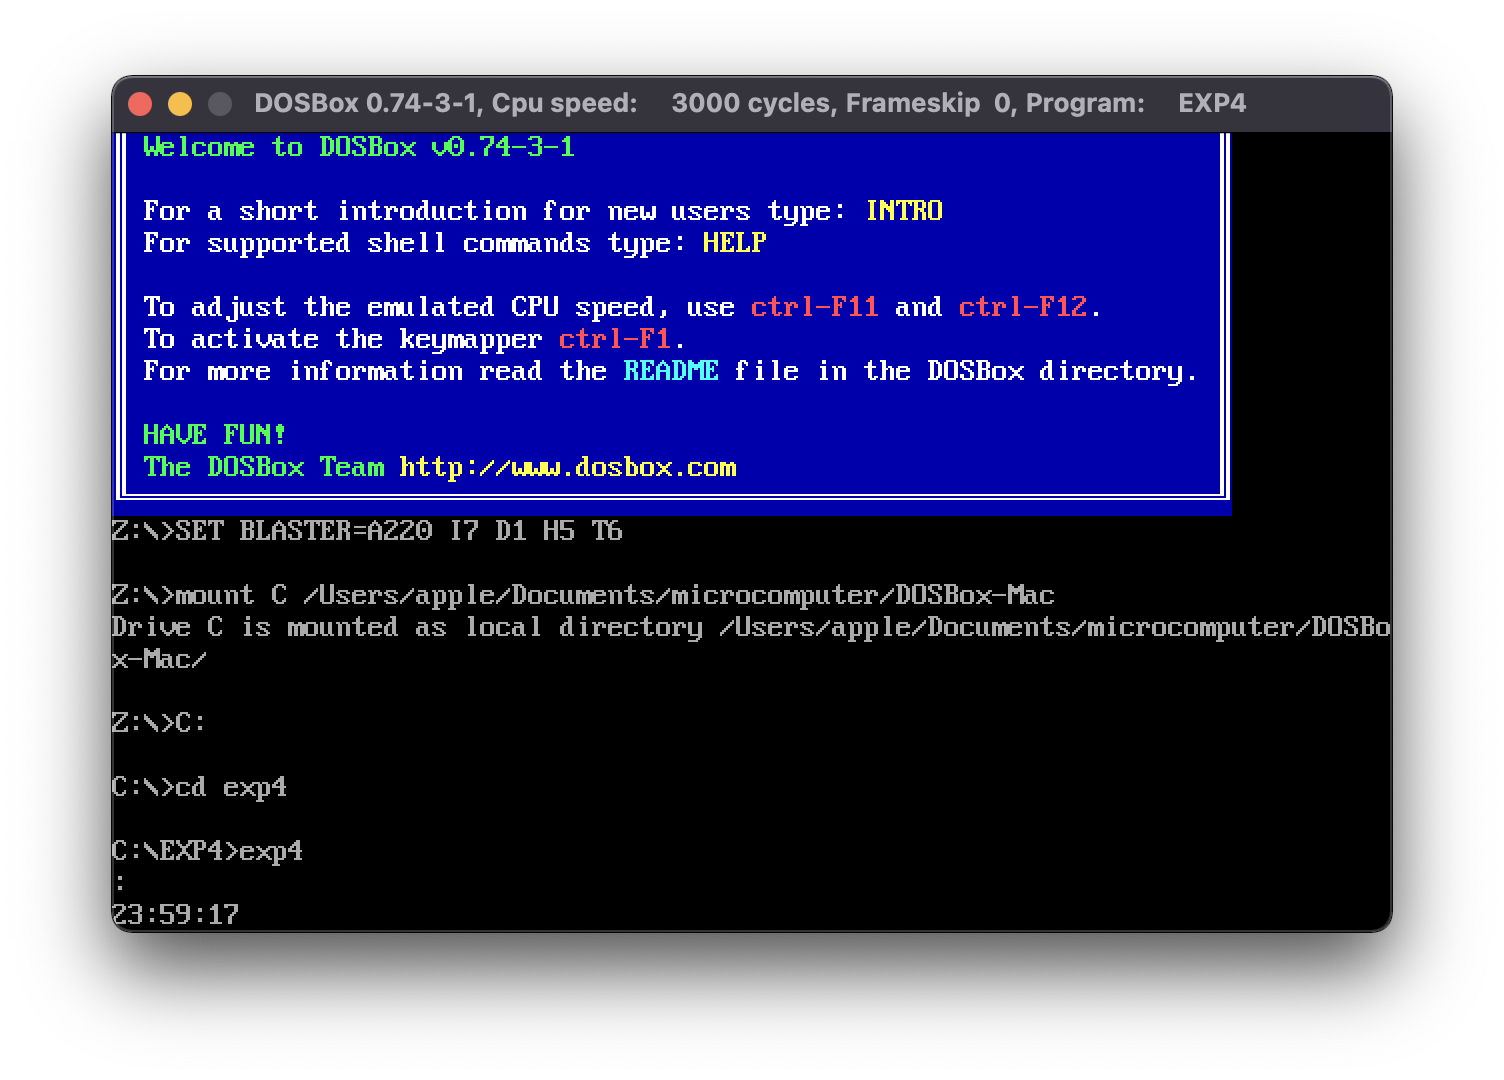
\includegraphics[width=0.7\textwidth]{fig/rlt00002.png}
    \caption{正确显示结果}
    \label{fig:right}
\end{figure}

\section{思考题}
\begin{table}[htbp]
    \centering
    \caption{思考 \label{tab:parameters}}
    \bgroup\def\arraystretch{1.5}
    \setlength{\tabcolsep}{4.5mm}
        \begin{tabular}{l}
          \toprule
          \textbf{实验思考题} \\
          \midrule\midrule
          \grayrow 时钟程序中存在时间误差吗?若有误差,其来源在何处?如何进行误差校正?\\
          \textcolor{red}{来源:}1.计算机设备自身的运行速度;\\
          2.第一次计时存在一些初始化和检测操作,这些操作在之后的计时中不需要,因此第一\\次计时和之后的计时之间有一定误差;\\
          3.延时1秒子程序无法十分精确地确定1秒钟,造成误差。\\
          \textcolor{red}{校正:}1.在延时1秒子程序中,调整循环程序代码执行的次数和循环程序中循环的次数,
          \\实现控制延时1秒的功能;\\
          2.可以通过调用系统时间进行校正。\\
          \bottomrule
        \end{tabular}
    \egroup
\end{table}


\section{附加任务描述及完成}
\subsection{附加任务1}
在同一行的相同位置显示更新的计时时间,不换行。
\begin{lstlisting}[language={[x86masm]Assembler},title=delay]
    DATA SEGMENT
    :
    :
    PRINT_ETR     DB 0DH,0AH,'$'        ;设置一回车输出串,
                                        ;在“:”显示后输出,换行缩进
    DATA ENDS
    :
    :
    MOV DL,':'                  ;显示时间输入提示符号“:”
    MOV AH,02H
    INT 21H
    LEA DX,PRINT_ETR            
    MOV AH,09H
    INT 21H
    :
    :
\end{lstlisting}

\begin{analyze}{换行显示问题}{}
    汇编里回车是回到本行首位,换行是到下一行同样位置。回车与换行的不同之处在于,换行会移到下一行,但‘回车+换行’却可以回到本行重新输出,这样,在待输出的字符串后面加上回车、换行符,即可实现同一行更新时间。
\end{analyze}

\subsection{附加任务2}
输入时间初值时,会检查是否有错、提示错误信息,并可重新输入时间初值。错误提示信息可以分两种:
\begin{enumerate}
    \item 输入的时间初值是错误的字符,即不是数字和冒号;
    \item 输入的时间值是错误的,即“时”大于等于24,“分”和“秒”大于等于60。
\end{enumerate}

\begin{lstlisting}[language={[x86masm]Assembler},title=delay]
    DATA SEGMENT
    :
    :
    WRONG_VALUE   DB 'Wrong value! Try again','$'                           ;错误类型1
    WRONG_NUMBER  DB 'The input must be colons or number! Try again','$'                           ;错误类型2
    DATA ENDS
    :
    :
    LENTH_TEST:                     ;长度测试
        MOV AL,TIME_IN+1            ;实际键入字数 
        CMP AL,08H                  ;和8比较,不相等跳转到 WRONG_INPUT
        JNE WRONG_INPUT_2
    FORMAT_TEST:                    ;格式测试
        MOV AL,TIME_IN+4            ;格式:XX:XX:XX
        CMP AL,':'
        JNE WRONG_INPUT_2
        MOV AL,TIME_IN+7
        CMP AL,':'
        JNE WRONG_INPUT_2
    INIT_LOW_LIMIT_TEST:
        LEA SI,TIME_IN+2
        MOV CL,03H                  ;循环3次
    LOW_LIMIT_TEST:
        MOV AL,[SI]		
        MOV AH,[SI+1]
        CMP AL,30H                  ;字符‘0’的ASCII码是30,不能小于0
        JB WRONG_INPUT_2            ;无符号小于则跳转
        CMP AH,30H                  ;字符‘0’的ASCII码是30,不能小于0
        JB WRONG_INPUT_2            ;无符号小于则跳转
        ADD SI,0003H
        LOOP LOW_LIMIT_TEST
    INIT_HIGH_LIMIT_TEST:
        LEA SI,TIME_IN+2
        MOV CL,03H
    HIGH_LIMIT_TEST:
        MOV AL,[SI]		
        MOV AH,[SI+1]
        CMP AL,39H                  ;字符‘9’的ASCII码是39,
                                    ;不能超过9,先得是个数字
        JA WRONG_INPUT_2            ;无符号大于则跳转
        CMP AH,39H                  
        JA WRONG_INPUT_2
        ADD SI,0003H
        LOOP HIGH_LIMIT_TEST
    HOUR_HIGH_TEST:
        MOV AL,TIME_IN+2
        CMP AL,32H                  ;字符‘2’的ASCII码是32,
                                    ;‘时’第一位不能超过2,
                                    ;‘分’和‘秒’同理
        JA WRONG_INPUT_1
    HOUR_FULL_HIGH_TEST:
        MOV AL,TIME_IN+3
        MOV AH,TIME_IN+2
        CMP AX,3233H                ;字符‘0204’的ASCII码是3233
        JA WRONG_INPUT_1
    MINUTE_TEST:
        MOV AL,TIME_IN+5
        CMP AL,35H
        JA WRONG_INPUT_1
    SECOND_TEST:
        MOV AL,TIME_IN+8
        CMP AL,35H
        JA WRONG_INPUT_1
        JMP INIT_IN                 ;检查完进行一个时间数值的调整
    WRONG_INPUT_1:
        LEA DX,WRONG_VALUE
        MOV AH,09H
        INT 21H
        JMP INPUT                   ;有错误需要重新输入
    WRONG_INPUT_2:
        LEA DX,WRONG_NUMBER
        MOV AH,09H
        INT 21H
        JMP INPUT                   ;有错误需要重新输入
    :
    :
\end{lstlisting}

\begin{analyze}{输入检查}{}
    输入检查原理是将相应字符\texttt{ASCII}码与数字比较,确保格式以及数值正确。
    \begin{note}{误区}{}
        检查数值过程需要逐位比较,例如在判断时候原先误将代码写为两位一起判断,如下
        \begin{lstlisting}[language={[x86masm]Assembler},title=code]
    MOV AL,[SI]		
    MOV AH,[SI+1]
    CMP AX,3030H            
    JB WRONG_INPUT_2       
        \end{lstlisting}
        这种情况下,如果非法字符的组合\texttt{ASCII}码大于\texttt{3030H}也可以通过检查,错误!
    \end{note}
\end{analyze}



\subsection{附加任务3}
延时一秒用\texttt{DOS}系统功能调用实现。

实验代码如下:
\begin{lstlisting}[language={[x86masm]Assembler},title=code]
    DELAY PROC NEAR                 ;延时1秒子程序     
        PUSH CX
        PUSH AX
        PUSH DX
        PUSH BX
        MOV AH,2CH                  ;读取当前时间,
                                    ;CH:小时;CL:分;DH:秒;
                                    ;DL:百分之一秒
        INT 21H
        MOV BH,DH                   ;将当前秒数存在BH中
        MOV AH,2DH                  ;设置时间
        INT 21H
    READ:
        MOV AH,2CH
        INT 21H
        CMP DH,BH                   ;比较两个时间的秒数,
                                    ;若相等则继续循环
        JE READ                     ;否则则经过了一秒
        POP BX
        POP DX
        POP AX
        POP CX
        RET
    DELAY ENDP   
\end{lstlisting}
\begin{analyze}{\texttt{Delay}程序说明}{}
    起初按照教材的方法设置延时过程,但是程序运行后时间变化非常快,更正后:判断循环时仅需与一秒进行比较即可,经过改正,成功实现了DOS调用。
\end{analyze}



\section{实验总结}
实验总结已随文附在“注意”、“思考”、“分析”中。

% 打印参考文献
\addcontentsline{toc}{section}{参考文献}
\printbibliography

\end{document}
